\chapter[Metodologia] {Metodologia}

O processo referente ao desenvolvimento do projeto Bibliotech terá como auxilio o Project Management Body of Knowledge (PMBOK), no que diz respeito à padronização na identificação e formação dos conceitos dos processos, será utilizado também na definição das áreas de conhecimento, ferramentas e técnicas presentes neste trabalho \cite{pmbok2004}

O fluxograma mostrado na figura abaixo apresenta como o projeto será implementado ao longo do semestre: 

\begin{figure}[!h]
\centering
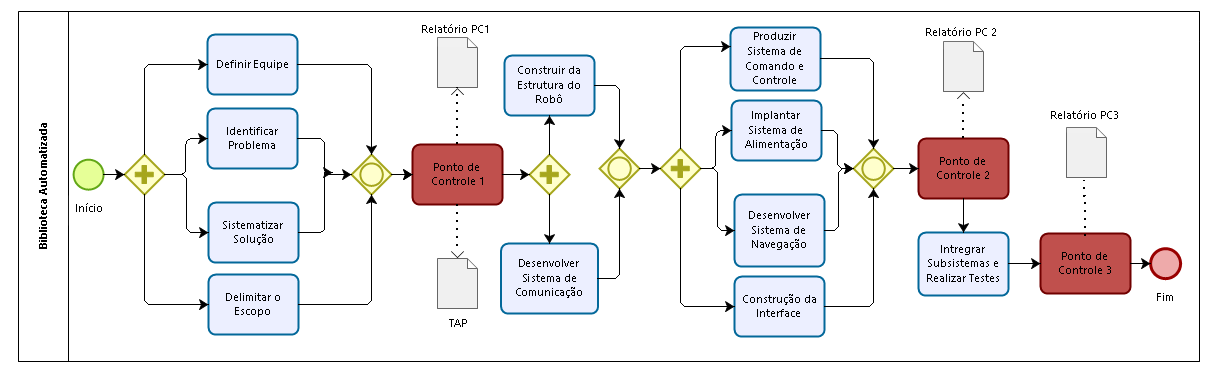
\includegraphics[scale=0.65, angle = 360]{figuras/fluxograma_metodologia}
\caption[]{Problema 02 (fonte: Autor)}
\end{figure}
\FloatBarrier

Pode-se observar que o projeto será divido em três pontos de controle que serão avaliados pelos professores da disciplina. No que tange o início do projeto deve-se realizar as seguintes tarefas descritas abaixo:

\begin{itemize}
\item Definir a Equipe: Esta etapa consiste na organização dos membros do projeto, tais como identificar os responsáveis por cada subsistema e delimitar os integrantes que irão trabalhar em conjunto para desenvolvê-los. Além da definição da política de comunicação do grupo, da metodologia de gerenciamento e como ocorrerão os encontros. 
\item Identificar Problema: Serão definidas as adversidades e obstáculos existentes em alguma situação, no caso uma biblioteca, para que se possa desenvolver um produto que apresente uma solução adequada para as contrariedades encontradas. Devem-se identificar também possíveis problemas que podem surgir no decorrer da criação do produto.
\item Sistematizar Solução: Após a identificação do problema, serão apresentadas possíveis soluções, no presente projeto a biblioteca automatizada, bem como as resoluções dos problemas relacionados a cada subsistema que constituem este produto.
Delimitar Escopo: Esta fase é constituída da definição dos objetivos e requisitos que o projeto deve cumprir.
\end{itemize}

Ao final dessas atividades para o Ponto de Controle 1 (PC1) deve-se apresentar toda a organização da equipe, metodologia de trabalho, o escopo bem definido, a solução planejada, de forma detalhada, e o plano de riscos do projeto. Após o cumprimento das atividades que compõem o Ponto de Controle 1 (PC1), dar-se-á início aos procedimentos para o Ponto de Controle 2(PC2), a seguir estão apresentadas as descrições das atividades:

\begin{itemize}
\item Construir a Estrutura do Robô e da Estante: No decorrer desta etapa está prevista a construção da estante, bem como a fabricação do mecanismo estrutural que será embutido nela. Deve-se, juntamente com a construção do robô, implementar como será feito o sistema de locomoção deste. Dado isso se pode dar início aos testes de resposta do robô aos comandos enviados pela raspberry.
\item Desenvolver Sistema de Comunicação: Implantação de um micro controlador para garantir que os parâmetros de tensão e corrente que serão fornecidos aos componentes do sistema estejam corretos.
\item Produzir Sistema de Comando e Controle: Nesta etapa será a integração da rede de comunicação entre a raspberry e o arduino, viabilizando o envio e recebimento de informações de ambos os componentes.
\item Implantar Sistema de Alimentação: A alimentação do equipamento será feita pela própria rede do local, logo esta etapa consiste na construção de um sistema de proteção, caso haja interrupção de fornecimento de energia, assim como o sistema de conversão.
\item Construção da Interface: Fase de implementação do sistema de comunicação entre o usuário e o computador que enviará os comandos para o robô.

No Ponto de Controle 2 deve-se apresentar os subsistemas funcionando separadamente possibilitando o início das tarefas que constituem o Ponto de Controle 3, onde começarão os testes de integração dos subsistemas objetivando a entrega do produto final. 

